\section{Super-Kamiokande and Atmospheric Neutrinos}
While the SNO experiment awas working to identify the source of the solar neutrino deficit, the Kamioka Nucleon Decay Experiment (KamiokaNDE) and its successor, Super-Kamiokande (Super-K), were using a similar water Cherenkov detector to search for proton decay.
The primary background for this rare process is neutrino interactions.
Unlike SNO, however, Super-Kamiokande was sensitive to both MeV solar neutrinos and higher energy GeV neutrinos produced in the atmospheric showers from cosmic ray interactions. 

\begin{figure}[!h]%
	\centering
		\subfloat[L/E From \cite{SuperK-Oscillations}]{
				\label{fig:superk_l_over_e}
				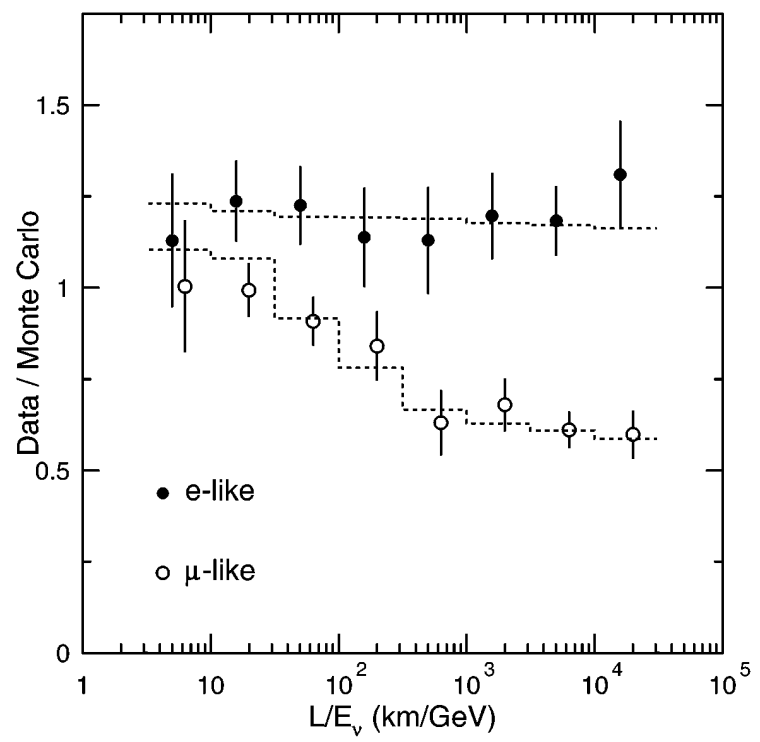
\includegraphics[width=0.5\linewidth]{superk_l_over_e.png}}%
		\subfloat[Oscillation Measurement from \cite{SuperK-Oscillations}]{
			\label{fig:superk_oscil}
			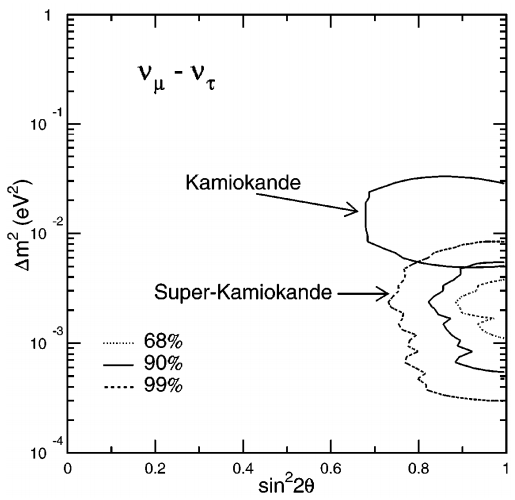
\includegraphics[width=0.5\linewidth]{superk_discovery.png}}%
	\caption{The first atmospheric neutrino oscillation measurements from the Super-K experiment. (a) The $\nu_e$-like events show no shape in L/E, as expected from a lack of neutrino oscillations. The $\nu_\mu$-like interactions, however, show a clear drop, indicating the presence of oscillation effects. (b) Using the two neutrino approximation, Super-K produced contours of the best-fit oscillation parameters for $\nu_\mu\rightarrow\nu_\tau$ oscillations. Both figures from \cite{SuperK-Oscillations}}%
\end{figure}


While investigating backgrounds, Super-Kamiokande observed an interesting deficit in the atmospheric neutrino signal.
Unlike the case in the solar neutrinos, the deficit observed by Super-K was observed solely in the muon neutrino events with no effect seem in the electron neutrinos \cite{SuperK-Oscillations}.
Using the reconstructed energy and direction of events, Super-K was able to show that the number of fully contained events of $\nu_\mu$-like interactions changed as a function of L/E - a clear signature of neutrino oscillations in the atmospheric neutrinos.
The figure, reproduced in Figure~\ref{fig:superk_l_over_e}, was used, in part, with an 2x2 approximation to the PMNS matrix to produce the first measurements, shown in Figure~\ref{fig:superk_oscil}, of the atmospheric oscillation parameters.
For the discovery of atmospheric neutrino oscillations at the same time as SNO's discovery of solar neutrino oscillations, the Super-K collaboration was jointly award the 2015 Nobel Prize \cite{NobelPrize:2015-Oscillations}.


